\begin{wrapfigure}[8]{l}{2.5cm}
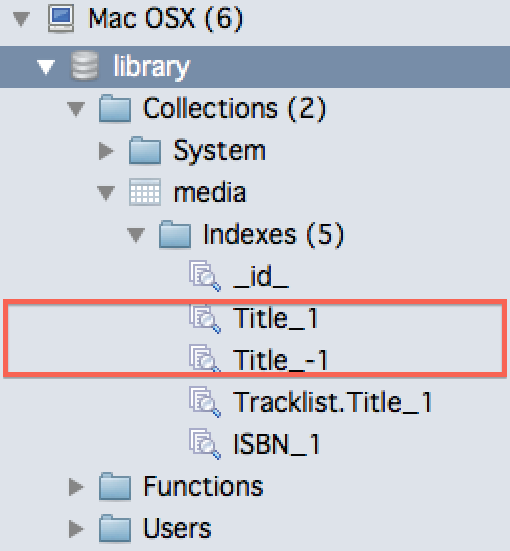
\includegraphics[scale=0.3]{img/indexes.png}
%\caption{The Universe}
\end{wrapfigure}
    \par
    Après la création de l’index avec la méthode ensureIndex un dossier arrive sous média indexes, l’index est définie au niveau de la collection associée. On y retrouve les objets index\_1 et index\_-1
    \begin{block}{Remarque}
        Sans index les recherches de type .find() ou .group() scan toute la collection. Elles font également appel, pour un large volume de data, au démon de mongodb : mongod. Ce qui est particulièrement lent. On créer alors des index pour faciliter la recherche sur les collections.
    \end{block}
    les indexes de mongodb respectent une organisation B-Tree\textsuperscript{4}… 
    \begin{block}{Note sur le model de donnée d'arbre en B}
    \newline
    C'est un model pour organiser des données de manière ordonnée. Il est sous forme d'arbre et grossit par la racine, c'est à dire que L’insertion des données (les clefs) se fait depuis le neud parent. Les clefs sont alors dirigées vers les neuds inférieures en fonction de leur valeur de sorte que le bout des branches soit ordonnée.    
    \end{block}
    \begin{figure}[h!]
    \centering
    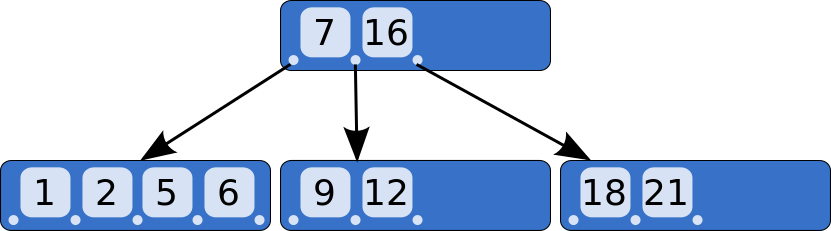
\includegraphics[scale=0.2]{img/btree.png}
    \caption{Représentation d"un arbre en B d"ordre 2.} 
    \end{figure}
    \par
    Pour faire le raprochement avec nos indexes mongodb, lindex Title\_1 correspond à la dernière ligne de l'arbre. c'est une suite de titres rangés dans l'ordre alphabétique dont chaqu'un a associé à un \_id.
    \begin{figure}[h!]
    \centering
    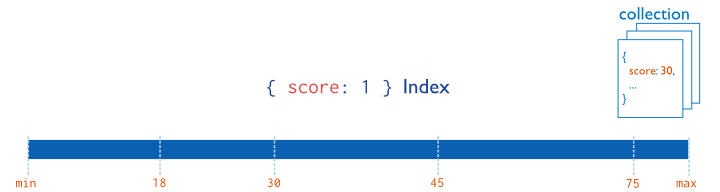
\includegraphics[scale=0.3]{img/indexmongodb.png}
    \caption{Binding entre l"index et la collection.\textsuperscript{5}}  
    \end{figure}
    \par
    La méthode .hint() force la recherche à l’aide d’un index. En indiquant des arguments on désigne un l’index approprié. Dans un premier temps lorsque l’index n’existe pas encore la ligne: \begin{tt}error:{"\$err": "bad hint", "code": 10113} \end{tt} nous indique une erreur. Une fois le l'index crée mongodb fait lien entre l'\_id indexé et le document de manière à pouvoir restituer des documents entiers.
    \begin{figure}[h!]
    \centering
    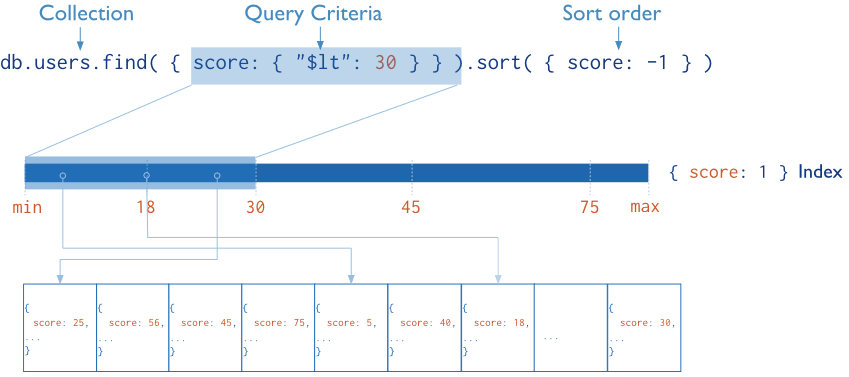
\includegraphics[scale=0.3]{img/indextocoll.png}
    \caption{Binding entre l'index et les documents de la collection\textsuperscript{5}} 
    \end{figure}

{\let\thefootnote\relax\footnotetext{\textsuperscript{4} \textit{\href{http://en.wikipedia.org/wiki/B-tree}{http://en.wikipedia.org/wiki/B-tree}}}}
        {\let\thefootnote\relax\footnotetext{\textsuperscript{5}\textit{Ressource images: \href{http://mongodb.org}{http://mongodb.org}}}}
